%!TEX root=main.tex
\chapter{Architecture}
\label{cha:architecture}

\chapterquote{We shape our buildings; thereafter they shape us.}{Winston Churchill, (1874 - 1965)}

Gilbert provides a Matlab-like language for distributed sparse linear algebra operations.
Being such a system, it comprises the complete stack of functionalities necessary to implement a programming language.
At first, the system has to divide the given source code into tokens.
These tokens are parsed and an abstract syntax tree (AST) is created.
In order to generate the intermediate representation (IR), it is necessary to assign types to the occurring expressions.
This assignment is done by the typing system.
Afterwards, the compiler can translate the Gilbert program into its IR.
The IR is well suited to apply high-level transformations to the program.
At last, the execution plan generator translates the IR into an execution plan which can be executed in parallel.

Since we had to implement the whole stack of functionalities of a programming language, Gilbert became quite complex.
In order to control this complexity, Gilbert's functionalities were separated into different layers with distinct tasks.
The layered system architecture is shown in \cref{fig:systemArchitecture}.
The separation of concerns limits the complexity of each layer so that each one of them becomes manageable.
In cooperation, though, they implement a highly elaborate system.

\begin{figure}
	\centering
	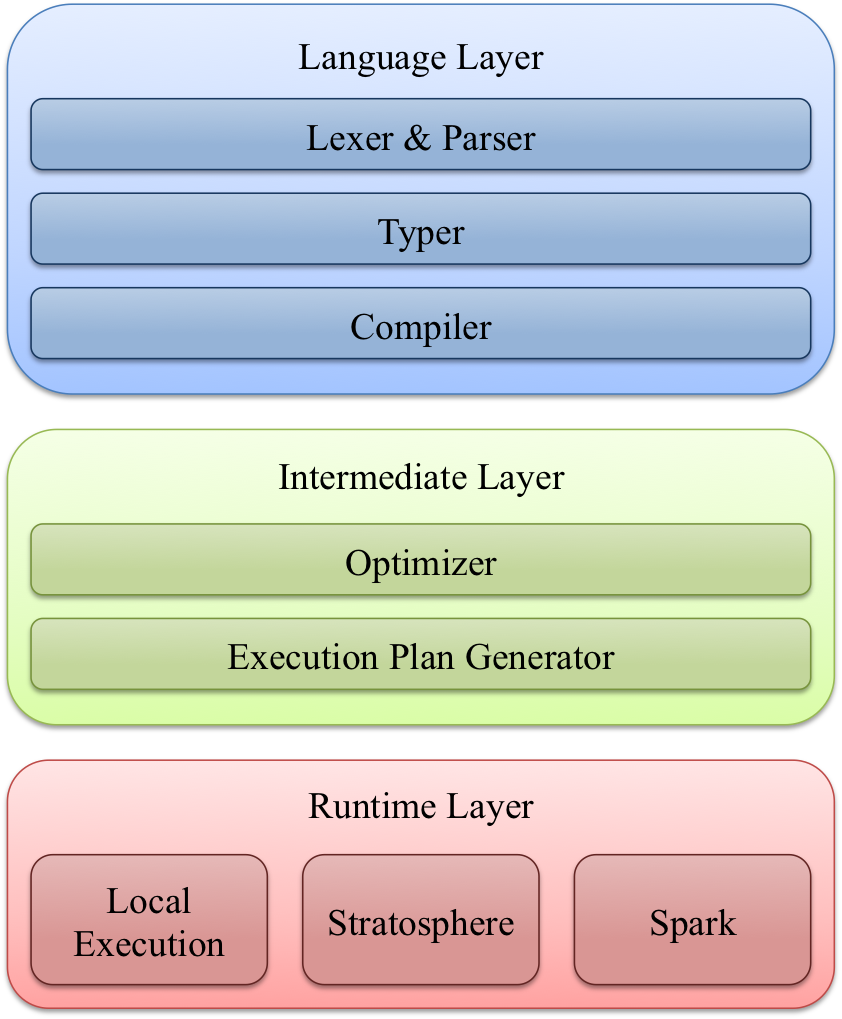
\includegraphics[width=0.5\linewidth]{images/systemArchitecture.png}
	\caption{The layered system architecture of Gilbert. The language layer is responsible for parsing, typing and compiling the given Matlab code. The intermediate layer facilitates high-level optimization strategies. The runtime layer is responsible for executing the specified program in parallel.}
	\label{fig:systemArchitecture}
\end{figure}

The first layer is the language layer.
It contains all functionality to parse the given Gilbert code and to compile it into the IR.
The second layer is the intermediate layer and it receives the IR of the Gilbert code.
The intermediate format is the ideal representation to apply language independent high-level transformations.
Consequently, the second layer hosts the optimizer.
The Gilbert optimizer applies several algebraic optimizations prior to the generation of the execution plan.
The execution plan generator translates the optimized IR into a specific execution plan, depending on the selected execution engine.
Once the program has been translated into an execution engine's specific plan, it is executed on the respective back end.

\section{Language Layer}

The language layer contains all the logic for translating Gilbert source code into the intermediate representation, see \cref{cha:intermediaterepresentation} for more details.
The layer itself is subdivided into three layers.
The first of these sublayers is the lexer and parser of MATLAB code.
Gilbert uses a recursive descent parser with backtracking, which is capable of parsing any LL(*) grammar.
Consequently, it can also parse Gilbert's front end language as specified in \cref{sec:languageGrammar}.

Once the MATLAB code is parsed, it is given to the next layer, namely the typing layer.
Here, the produced AST is attributed with type information.
This information is inferred automatically from the source code without any need for explicit type annotations.
The typer makes use of the Hindley-Milner type inference system, as it is described in \cref{sec:hmInference}.
After the types have been inferred, a new AST with additional type information is generated.

The type information enriched AST is given to the last sublayer.
The compiler is responsible for translating the AST into a front end independent representation of linear algebra operations, namely the IR.
The format Gilbert uses to represent linear algebra operations in a generalized format is described in \cref{cha:intermediaterepresentation}.
In fact, it is also some form of AST just without the peculiarities of MATLAB.

\section{Intermediate Layer}

The intermediate layer contains the optimizer and the execution plan generator.
The optimizer works on the intermediate representation of the Gilbert program.
It applies the optimizations described in \cref{cha:optimizer}.
The execution plan generator's task is to translate the intermediate format into the execution engine's specific format.
Currently, the system supports local execution and two engines for distributed execution, namely Stratosphere and Spark.

For the local execution, Gilbert employs an interpreter.
The interpreter directly executes the intermediate representation.
Beginning at the root of the dependency tree, the interpreter utilizes a recursive-descent strategy to evaluate each node.
In order to evaluate a given node of the tree, the interpreter first descends to its children.
After having retrieved the results of the children nodes, the parent node is evaluated.

The distributed execution engines do not support immediate execution of the individual nodes.
Instead, the plan generator has to create an execution plan for Stratosphere and Spark, which is lazily executed upon submission or when Spark's actions are called.
Fortunately, Stratosphere and Spark offer a similar programming API.
Thus, Gilbert can translate the distinct linear algebra operations using the same general building blocks as described in \cref{sec:LinearAlgebraOperations}.
The execution plan is generated using a recursive-descent approach similar to the local interpreter.
Once the intermediate representation has been transformed, the plan is sent to the respective system.
The system is responsible for the parallel execution.

\section{Runtime Layer}

The runtime layer marks the transition from Gilbert to one of the supported execution engines.
It is more of a conceptual abstraction of the Gilbert system.
Gilbert supports 3 different engines at the moment, but it should be easy to add support for further execution systems.
